% Figure 1, panel G: what SPARK returns, from a real run rather than a cartoon.
% The contents are produced by figures/fig1_panelG.py, which reads DAG 3 of the
% simulation study under the expert-elicited prior through the loaders in
% results_simulation/figures/config.py, and writes figures/fig1_panelG.pdf via
% matplotlib's pgf backend so its type is the same Computer Modern as the rest of
% the figure. Regenerate with:
%     python3 figures/fig1_panelG.py
% DAG 3 rather than DAG 7 on purpose: Figure 2 features DAG 7, and reusing it here
% would make this panel's matrix a duplicate of Figure 2C.
% Local origin is the panel's top-left corner. Panel size 16.4 x 6.35: the
% included graphic is 5.65 cm tall, set below the panel letter at 0.52 and
% clearing the frame by 0.18 at the foot.
\draw[panel] (0,0) rectangle (16.4,-6.35);
\node[ttl] at (0.15,-0.12) {G\quad What SPARK returns};

% Shift measured with the frame and the panel letter excluded, so the
% drawing sits centred in the space below the letter rather than wherever
% its coordinates happened to put it.
\begin{scope}[shift={(-0.007,-0.048)}]  % centre the panel contents


\node[anchor=north west, inner sep=0pt] at (0.25,-0.52)
  {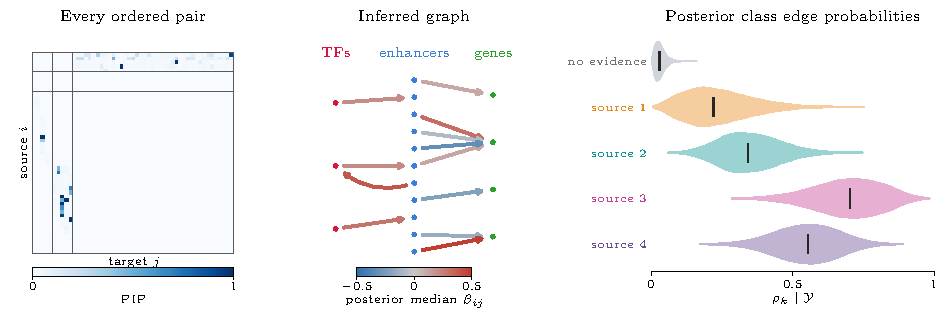
\includegraphics[width=15.9cm]{figures/fig1_panelG}};
\end{scope}
